\documentclass[aspectratio=169]{beamer}
\usetheme{boxes}
\usepackage{essay-def}
\usepackage{bm}
\usepackage{amsfonts}
\usepackage{amssymb}
\usepackage{amsmath}
\usepackage{amsthm}
\usepackage{comment}
\usepackage{subcaption}
\usepackage{geometry}
\usepackage{algorithmic}
\usepackage{algpseudocode}
\usepackage{algorithmicx}
\geometry{left=1cm,right=1cm}
    \title[Probabilistic SGS modeling]{A probabilistic approach to 
		subgrid-scale modeling}
\author[J. Zhao]{Jiaxi Zhao \\ \small joint with Sohei Arisaka and Qianxiao Li @ NUS}
\date[\today]{AI4X \\ \today}
\begin{document}
\par \setlength{\parindent}{2em}

\begin{frame}
\titlepage
\end{frame}


% \geometry{left=1cm,right=1cm}
%     \title[Probabilistic SGS modeling]{Algorithmic development for data-driven 
% 		hybrid simulations}
% \author[J. Zhao]{Jiaxi Zhao \\ \small joint with Sohei Arisaka and Qianxiao Li @ NUS}
% \date[\today]{AI4X \\ \today}
% \begin{document}
% \par \setlength{\parindent}{2em}

% \begin{frame}
% \titlepage
% \end{frame}


% \begin{frame}{An abstraction of SciML workflow}
% 	Simulating the dynamics:
% 	\bequn
% 		\begin{aligned}
% 			\mcL(\mfu, \p_t \mfu, \mfy, t) & = \mathbf{0}, \quad \mfu \in \mcU, \mfy \in \mcY, \mcL: \mcU \times T\mcU \times \mcY \times \mbR_+ \rightarrow \mbR^{n},			\\
% 			\mfy & = \phi(\mfu, t), \quad \phi: \mcU \times \mbR_+ \rightarrow \mfy.
% 		\end{aligned}
% 	\eequn
% 	\begin{itemize}
% 		\item 1. $\mcL$ is known, possibly non-linear, {\color{red}while $\phi$ is un-known.}
% 		\item 2. Datasets: $\lbb (\mfu_1, \mfy_1, t_1), (\mfu_2, \mfy_2, t_2), \cdots, (\mfu_N, \mfy_N, t_N )\rbb. $
% 		\item 3. {\color{red} Benchmark algorithm solves the ordinary least square:
% 		\bequn
% 			\arg\min_{\theta} \mbE \norml \mfy - \phi_{\theta}(\mfu, t) \normr^2.
% 		\eequn}
% 	\end{itemize}
	
% 	Typical examples: subgrid-scale modeling, reynolds stress modeling, exchange-correlation functional.

% \end{frame}


% \begin{frame}{A-priori and a-posteriori discrepancy}
% 	The inconsistency between the a priori error and a posteriori error arises because the {\color{red}training algorithm does not take the solver dynamics into account}.
% 	\begin{figure}
% 		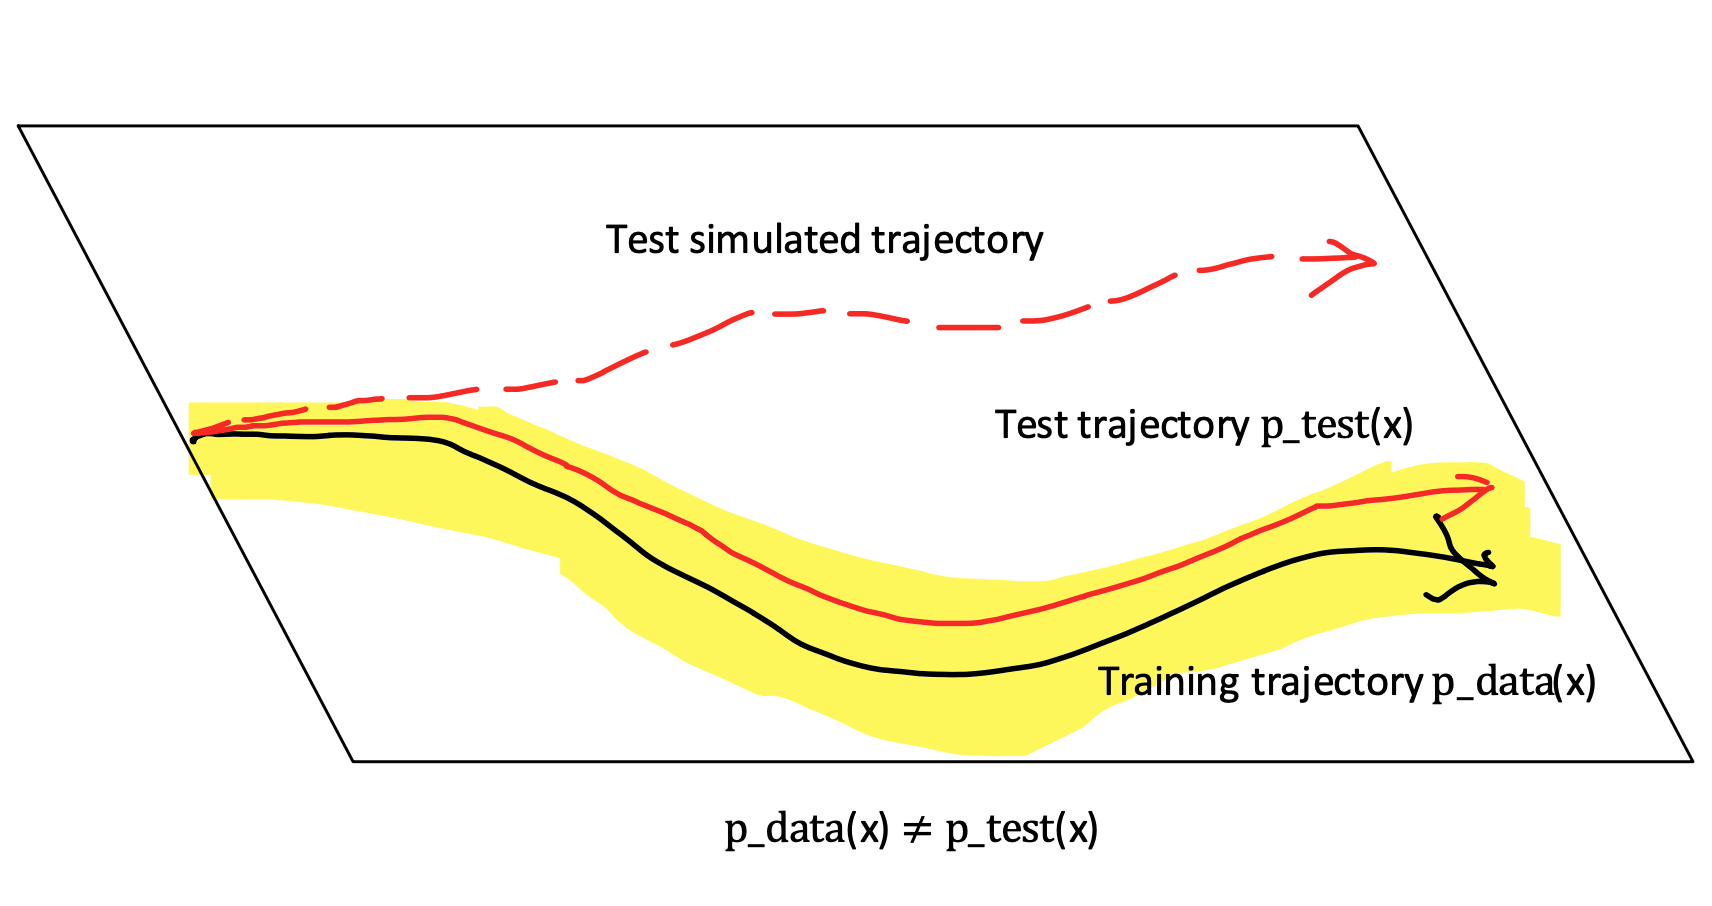
\includegraphics[width=.6\textwidth]{fig/dilemma.png}
% 		\label{fig:dilemma}
% 	\end{figure}
% \end{frame}


% \begin{frame}{Alg 1: Manifold regularization}
% 	Regularization encodes the information of the data manifold.
% 	\begin{figure}[H]
% 		\centering
% 		\centerline{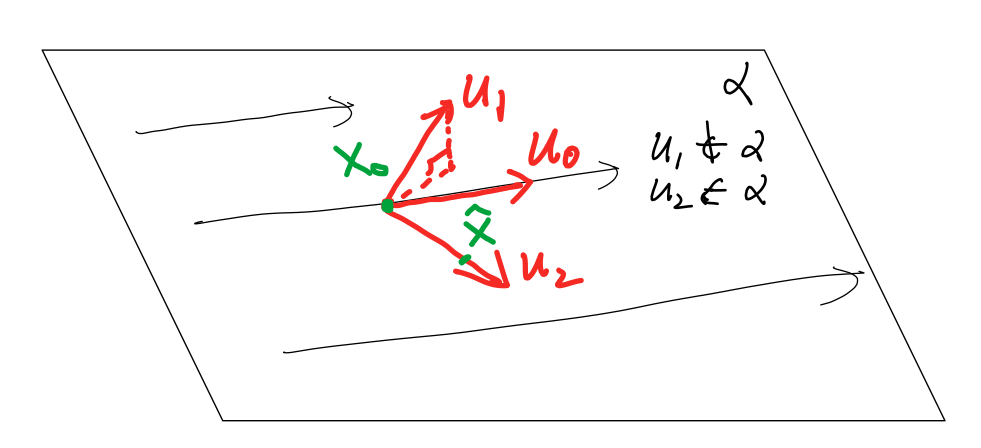
\includegraphics[width=0.9\linewidth]{fig/mfd.png}}
% 	\end{figure}
% 	\begin{equation*}
% 		l_{\text{TR}}(\theta) := \mbE_{(\mfu, \mfy)}\lb \norml \mfy_k - \phi_{\theta}(\mfu) \normr_2^2
% 		+ \lambda \lp\lp  \nabla F(\mfu) \rp^T L(\mfu, \phi_{\theta}(\mfu), t)\rp^2 \rb.
% 		\end{equation*}
% 	\footnotetext[1]{Zhao, Jiaxi, and Qianxiao Li. "Mitigating Distribution Shift
% 	in Machine Learning–Augmented Hybrid Simulation." SIAM Journal on
% 	Scientific Computing 47.2 (2025): C475-C500.}
% \end{frame}


% \begin{frame}{Alg 2: Probabilistic ansatz}
% 	Regression to generative modeling:
% 	\begin{equation*}
%     \tau = \phi_{\theta}(\mfu) \quad \rightarrow \quad \tau \sim p_{\theta}(\cdot|\mfu).
% 	\end{equation*}

% 	Change of the loss functions:
% 	\begin{equation*}
%    \min_{\theta} \sum_{n} \norml \phi_{\theta}(\wtd{\mfu}^{(n)}) - \tau^{(n)} \normr^2,\quad
% 	 \max_{\theta}\sum_{i=n}^{N}\log p_{\theta}(\tau^{(n)}|\mfu^{(n)}).
% 	\end{equation*}
% 	\footnotetext[2]{Zhao, Jiaxi, Sohei Arisaka, and Qianxiao Li. 
% 	"Generative subgrid-scale modeling." ICLR 2025 Workshop on Machine
% 	Learning Multiscale Processes.}
% \end{frame}


% \begin{frame}{Alg 3: Correction-based SGS models}
% 	Considering a PDE with both linear and nonlinear terms
% 	\begin{equation*}
% 		\partial_t \overline{u} + \mathcal{L}(\overline{u}) + \mathcal{N}(\overline{u}) + \tau(\overline{u}) = 0.
% 	\end{equation}
% 	\begin{itemize}
% 		\item Filter-based approach:
% 		\begin{equation*}
% 			\mathcal{F}(u^f) = u^c \Longrightarrow \tau^{(1)} = 
% 			\mathcal{F}(\mathcal{N}(u^f)) - \mathcal{N}(u^c).
% 	\end{equation*}
% 		\item Correction-based approach:
% 		\begin{equation}
% 			\mathcal{F}(u^f) = u^c \Longrightarrow \tau^{(2)} =
% 			\mathcal{F}(\text{solver}^f(u^f)) - \text{solver}^c(u^c),
% 	\end{equation}
% 	\end{itemize}
	
% \end{frame}


% \begin{frame}{Content}
% 	\begin{itemize}
% 		\item 1. Difficulties encountered in the data-driven turbulence modeling.
% 		\item 2. Possible explanation of the problem on 1D Kuramoto–Sivashinsky
% 		equation.
% 		\item 3. An effective probabilistic SGS model that improves the
% 		regression-based method.
% 	\end{itemize}
% \end{frame}


\begin{frame}{Fluid simulations in real world}
	% \begin{itemize}
	% 	\item 1. Performing DNS is unaffordable, even a LES with 50M grids of length 1000s takes several days.
	% 	\item 2. Cheap simulation such as RANS and coarse-grid LES can not obtain accurate quantities such as peak pressure.
	% \end{itemize}

	Full-resolution simulations are unaffordable for climate and
	urban environment modeling.
	\begin{figure}[ht]
		\centering
		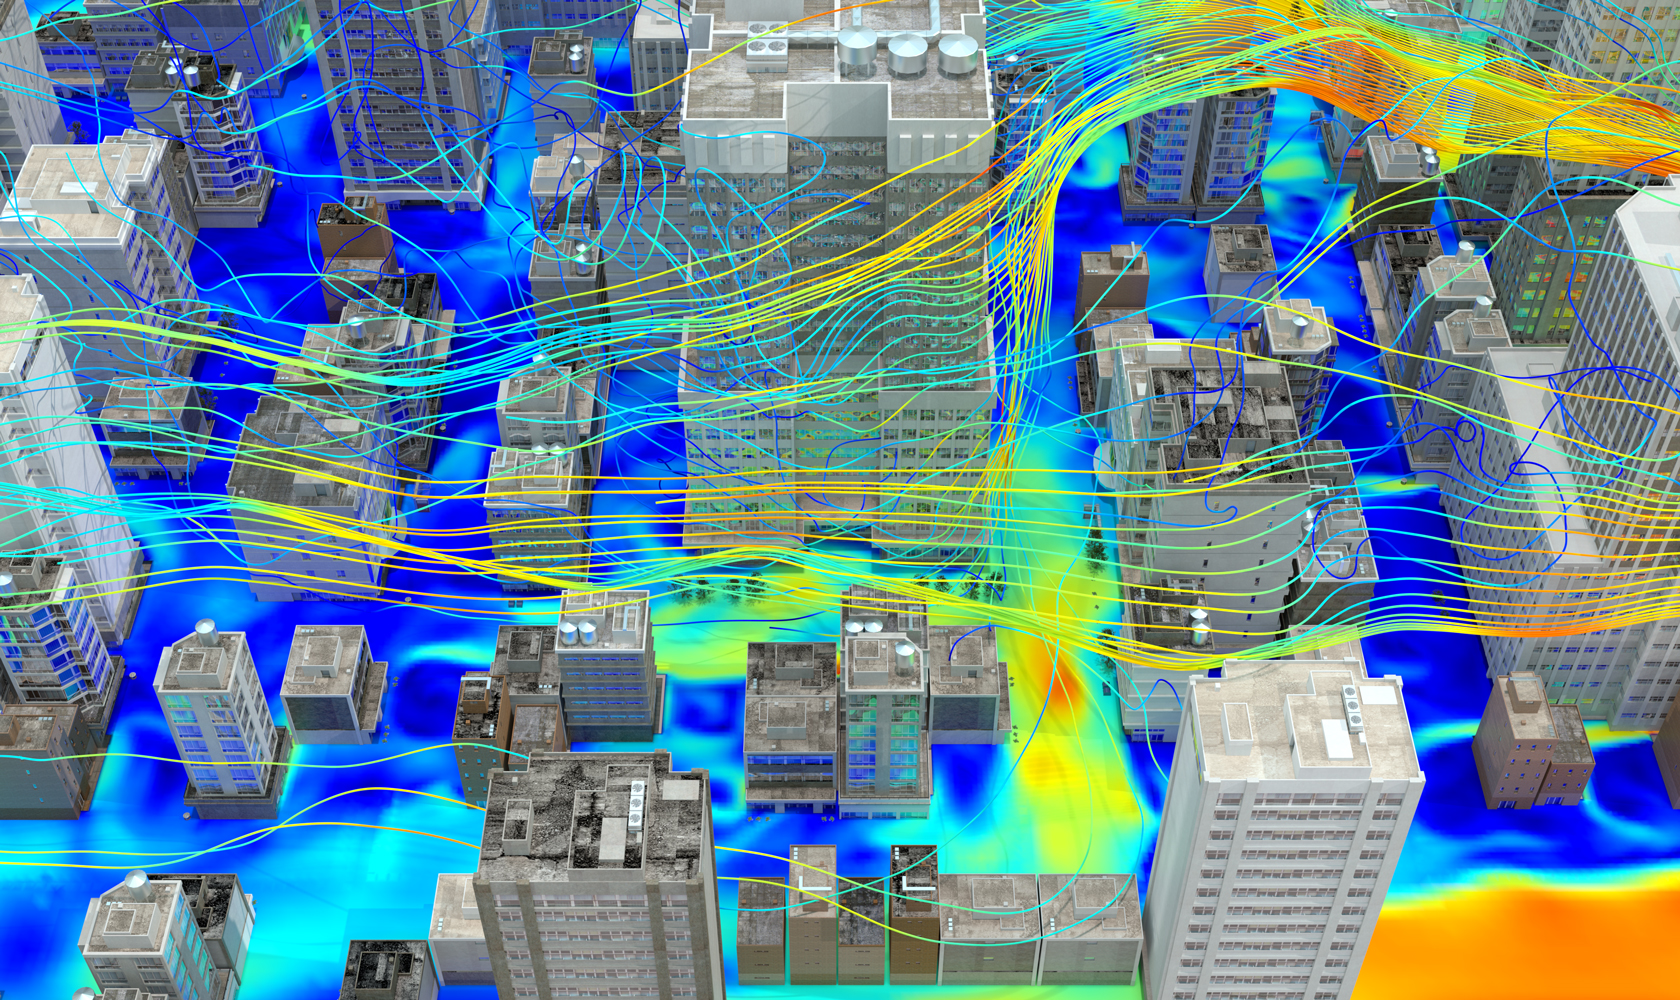
\includegraphics[width=.6\linewidth]{fig/urban_environment.jpeg}
	\end{figure}

	\textit{Can we {\color{red}design or learn better SGS models} based on
 the fine-grid simulation data
 so that it can achieve accurate results even {\color{red}on coarse grid 
 simulations?}}
\end{frame}


\begin{frame}{A primer on SGS modeling}
	\begin{equation*}
		\begin{aligned}
		\frac{\p u_i}{\p t} + \frac{\p}{\p x_j}(u_iu_j) & \ = 
		-\frac{\p p}{\p x_i} + \nu\Delta u_i,   \\
		\frac{\p u_i}{\p x_i} & \ = 0.
		\end{aligned}
	\end{equation*}

	\textbf{\color{red}Applying a filter $G$ to the equation}, i.e. 
	$\overline{u} = G * u$ (rough to smooth)
	\begin{equation*}
		\begin{aligned}
		\frac{\p \overline{u}_i}{\p t} + \frac{\p}{\p x_j}(\overline{u}_i
		\overline{u}_j) & \ = -\frac{\p \overline{p}}{\p x_i} + \nu\Delta 
		\overline{u}_i - \frac{\p \tau_{ij}}{\p x_j},   \\
		\frac{\p \overline{u}_i}{\p x_i} & \ = 0,		\\
		\overline{\mathbf{u}} \longrightarrow \tau_{ij} & \ = \overline{u_iu_j} - \overline{u}_i\overline{u}_j.
		\end{aligned}
	\end{equation*}

	Classical SGS stress models include the (dynamic) Smagorinsky model, 
	and the Wall-Adapting Local Eddy-Viscosity model, and etc. They all based
	on physical intuition and empirical data.
\end{frame}


\begin{frame}{Pipeline of Data-driven SGS modeling}
	\begin{itemize}
		\item 1. Conduct fine-grid simulations and apply filter to obtain data pair of
		filtered-velocity and SGS stress.
		\item 2. Train a SGS model.
		\begin{equation*}
			\min_{\phi}\norml \tau - \phi(\overline{\mathbf{u}}) \normr^2.
		\end{equation*}
		\item 3. Deploy the model in the simulation.
		\begin{equation*}
			\begin{aligned}
			\frac{\p \overline{u}_i}{\p t} + \frac{\p}{\p x_j}(\overline{u}_i
			\overline{u}_j) & \ = -\frac{\p \overline{p}}{\p x_i} + \nu\Delta 
			\overline{u}_i - \frac{\p \phi(\overline{u})_{ij}}{\p x_j},   \\
			\frac{\p \overline{u}_i}{\p x_i} & \ = 0.
			\end{aligned}
		\end{equation*}
	\end{itemize}

	\textbf{\color{red} We care more about the performance of the SGS model in
	simulation (a-posteriori performance) than 
	training loss (a-priori performance).}
\end{frame}


\begin{frame}{Existing modeling approaches}
	\begin{itemize}
		\item 1. Rely on classical turbulence models, e.g. Smagorinsky model and
		use DNS data to fit the model parameters.
		\begin{equation*}
			\tau = C_{\theta}(\overline{\mathbf{u}})||S||^2 S, \quad S = \nabla \overline{\mathbf{u}} + \nabla \overline{\mathbf{u}}^T.
		\end{equation*}
		\item 2. Choose the input features and fit an end-to-end mapping between
		them and the QoI.
		\begin{equation*}
			\tau = \phi_{\theta}(\overline{\mathbf{u}}).
		\end{equation*}
		\item 3. View the SGS stress modeling as a policy and solve it in the
		framework of reinforcement learning.
	\end{itemize}
\end{frame}


% \begin{frame}{SGS stress modeling}
% 	There are three main issues for stress modeling:
% 	\begin{itemize}
% 		\item 1. The mapping from the input features. e.g. filtered velocity to the
% 		stress tensor is {\color{red}non-deterministic} while
% 		most classical turbulence models and data-driven models are deterministic.
% 		\begin{equation*}
% 			\overline{u}, \nabla \overline{u}, \overline{p} 
% 			\overset{\text{NOT DETERMINISTIC}}{\Longrightarrow} \tau, \quad 
% 			\min_{\phi}\norml \tau - \phi(\overline{u}) \normr^2.
% 		\end{equation*}
% 		\item 2. Discrepancy between 
% 		{\color{red}a-priori error and a-posteriori error}.
% 		\begin{equation*}
% 			\norml \wht\tau - \tau \normr^2, \quad \norml \overline{u}(T) -
% 			\overline{u}(T) \normr^2
% 		\end{equation*}
% 		This is very different from classical numerical analysis perspective where
% 		a smaller truncation error (higher order) mostly indicates faster
% 		convergence via the Lax equivalence theorem.
% 		\item 3. Difficult to combine the OpenFOAM solver with gradient-based
% 		optimization algorithms.
% 	\end{itemize}
% \end{frame}


\begin{frame}{A-priori and a-posteriori discrepancy}

	The inconsistency between the a priori error and a posteriori error
	arises because the {\color{red}training algorithm does not take the
	solver dynamics into account}.
	\begin{figure}
		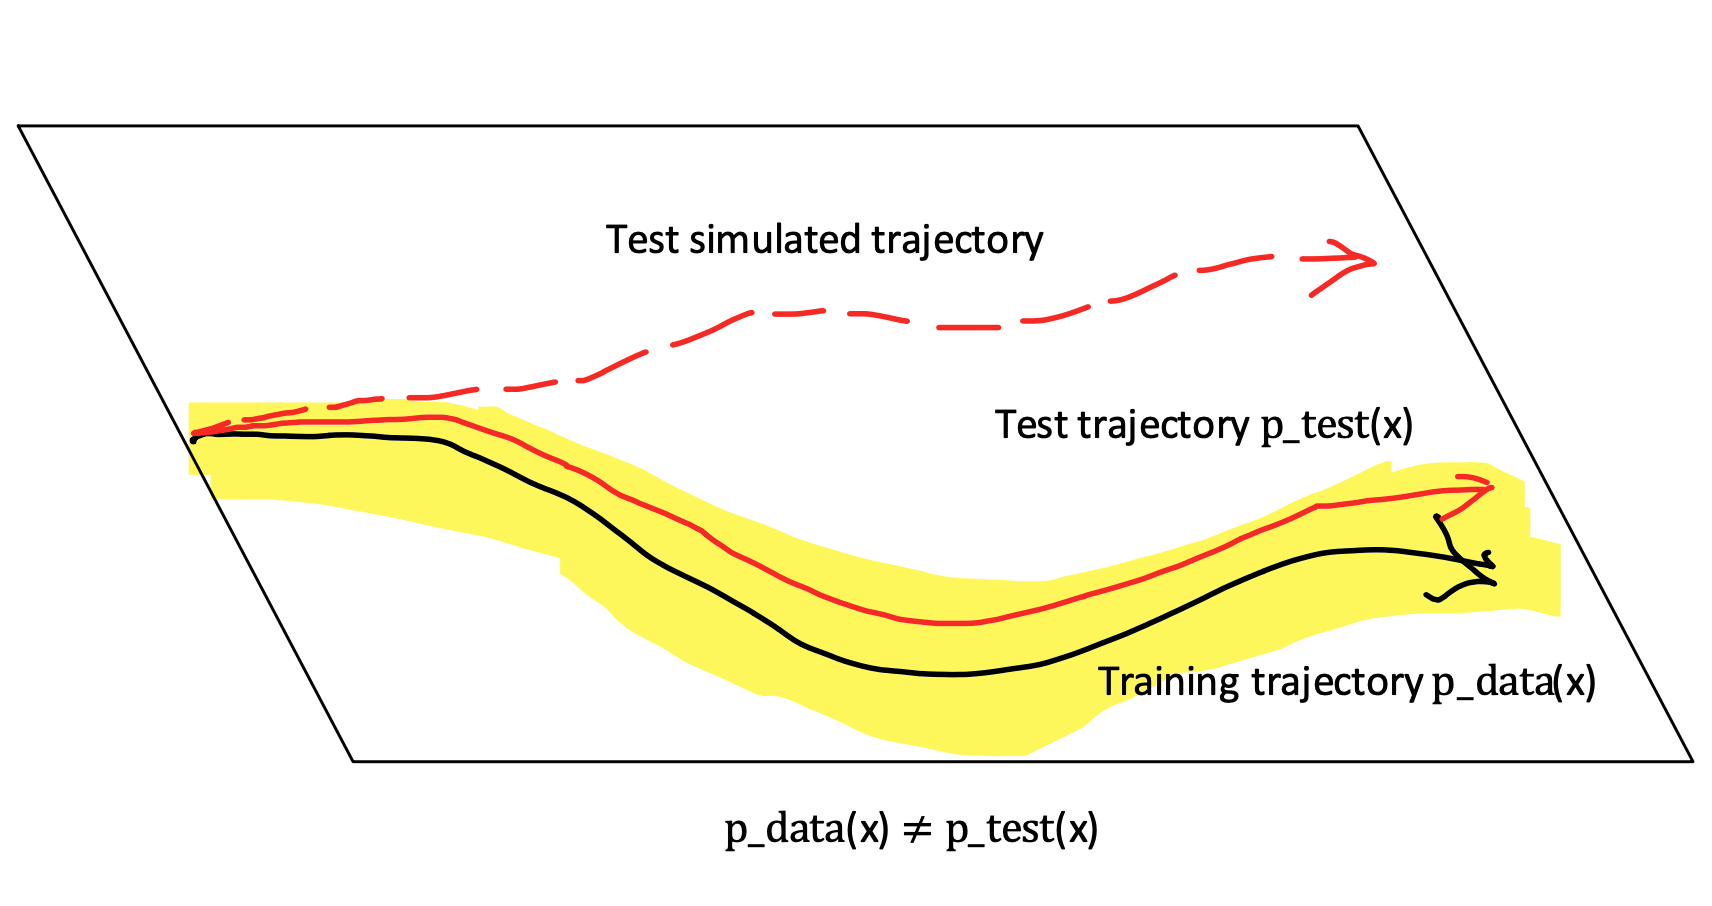
\includegraphics[width=.6\textwidth]{fig/dilemma.png}
		\label{fig:dilemma}
	\end{figure}
	\begin{figure}
		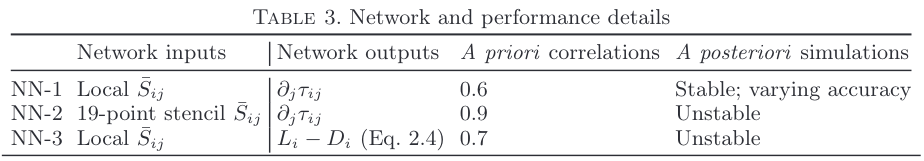
\includegraphics[width=.8\textwidth]{fig/dichotomy.jpg}
		\label{fig:dichotomy}
	\end{figure}
\end{frame}


\begin{frame}{Visualizing SGS modeling: KS equation}

	1D toy model: Kuramoto–Sivashinsky equation.
	\begin{equation*}
		\begin{aligned}
			u_t & = -(c + u)u_x - uu_x - u_{xx} - \nu u_{xxxx},    \\
			u(0, t) & = u(L, t) = 0, \\
			u_x(0, t) & = u_x(L, t) = 0, \forall t. \\
		\end{aligned}
	\end{equation*}
	
	\begin{itemize}
		\item 1. Fine-grid simulation: $u_{1024}$;
		\item 2. Restriction operator: $\opP$ to coarse grid;
		\item 3. Filtered variables: $u_{256} = Pu_{1024}$.
		\item 4. SGS stress:
		$$\tau_{256} = \opP(u_{1024}^2) - (\opP u_{1024})^2.$$
	\end{itemize}
\end{frame}


\begin{frame}{Multivalue issue}

	Both $\mathbf{u}$ and $\tau$ are 1D, scatter to visualize them.
	\begin{figure}[ht]
		\centering
		\begin{subfigure}[b]{\textwidth}
			\centering
			
\includegraphics[width=.7\textwidth]
			{fig/regression_uxx_tau_err_scatter.png}
		\end{subfigure}
		\begin{subfigure}[b]{\textwidth}
			\centering
			
\includegraphics[width=.7\textwidth]
			{fig/regression_uxxxx_tau_err_scatter.png}
		\end{subfigure}
	\end{figure}

	\textbf{\color{red} Same input can produce different outputs.}
\end{frame}


% \begin{frame}{A priori and a posteriori}
% 	\begin{figure}[ht]
% 		\centering
% 		\begin{subfigure}[b]{0.32\textwidth}
% 			\centering 
% 			\includegraphics[width=\textwidth]
% 			{fig/ks_nu0.1_N1512N2256_correct_cmp_lr1e-4.pdf} 
% 			\caption{validation loss: 3.5000e-05} 
% 		\end{subfigure}
% 		\begin{subfigure}[b]{0.32\textwidth}
% 			\centering 
% 			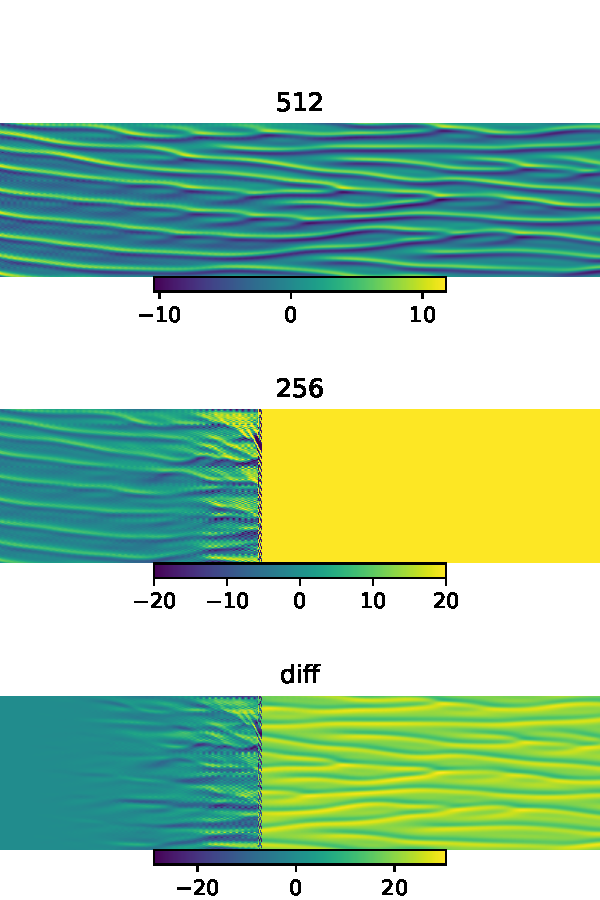
\includegraphics[width=\textwidth]{fig/ks_nu0.1_N1512N2256_correct_cmp_lr2e-4.pdf} 
% 			\caption{validation loss: 1.3050e-05} 
% 		\end{subfigure}
% 		\begin{subfigure}[b]{0.32\textwidth}
% 			\centering 
% 			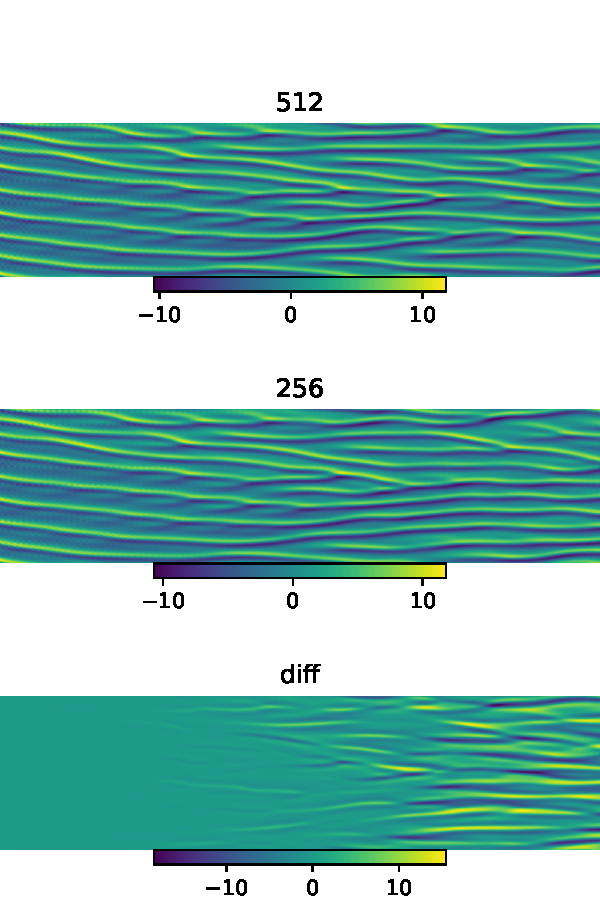
\includegraphics[width=\textwidth]{fig/ks_nu0.1_N1512N2256_correct_cmp_lr5e-4.pdf} 
% 			\caption{validation loss: 2.8155e-05}  
% 		\end{subfigure}
% 	\end{figure}
% \end{frame}


\begin{frame}{Solution: Probabilistic ansatz}

	Regression to generative modeling:
	\begin{equation*}
    \tau = \phi_{\theta}(\mfu) \quad \rightarrow \quad \tau \sim p_{\theta}(\cdot|\mfu).
	\end{equation*}

	Change of the loss functions:
	\begin{equation*}
   \min_{\theta} \sum_{n} \norml \phi_{\theta}(\wtd{\mfu}^{(n)}) - \tau^{(n)} \normr^2,\quad
	 \max_{\theta}\sum_{i=n}^{N}\log p_{\theta}(\tau^{(n)}|\mfu^{(n)}).
	\end{equation*}
	\footnotetext[2]{Zhao, Jiaxi, Sohei Arisaka, and Qianxiao Li. 
	"Generative subgrid-scale modeling." ICLR 2025 Workshop on Machine
	Learning Multiscale Processes.}
\end{frame}


\begin{frame}{Optimizing the model}

	Instead of using the MSE as the loss function, we optimize our model by
	maximize the likelihood over data:
	\begin{equation*}
		\begin{aligned}
			\min_{\theta} &\sum_{i=1}^{N}\frac{(y_i - \mu_{\theta}(x_i) )^2}
			{2(\sigma_{\theta}(x_i))^2} + \log \sigma_{\theta}(x_i),		\\
			\min_{\theta} &\sum_{i=1}^{N}-\log\lp \sum_{j=1}^M \frac{\text{softmax}
			(c_{\theta}^j(x_i))}{\sigma_{\theta}^j(x_i)}
			\exp\lb-\frac{(y_i - \mu_{\theta}^j(x_i) )^2} 
			{2(\sigma_{\theta}^j(x_i))^2} \rb\rp.
		\end{aligned}
	\end{equation*}

	Currently, we naively use the Adam solver to optimize this non-linear
	optimization problem.
\end{frame}


\begin{frame}{Integrating in the simulation}

	How can we deploy this model in the simulation?
	\begin{equation*}
		\begin{aligned}
			\text{Gaussian: } u_i & \Longrightarrow \mu_{\theta}(u_i), \sigma_{\theta}(u_i),
			z \sim N(0, 1), \\
			\tau_{ij} & = \mu_{\theta}(u_i) + \sigma_{\theta}(u_i)z,	\\
			\text{Gaussian mixture: } u_i & \Longrightarrow \mu_{\theta}^j(u_i), \sigma_{\theta}^j(u_i),
			z \sim N(0, 1), j \sim [M], \\
			\tau_{i} & = \mu_{\theta}^j(u_i) + \sigma_{\theta}^j(u_i)z,	\\
		\end{aligned}
	\end{equation*}

	There is temporal and spatial consistency issue. Should we use the same
	latent variable $z$ for all the grid points at all the time step or we
	should use different $z_i$ for different $u_i$?
\end{frame}


% \begin{frame}{Comparison with the regression-based method}
% 	\begin{equation*}
% 		\begin{aligned}
% 			\la\overline{u}\ra &= \frac{1}{LT}\int_{[0, L]}\int_{t}^{t+T} u(x, t)dt dx,
% 			\\
% 			\la\overline{u^2}\ra &= \frac{1}{LT}\int_{[0, L]}\int_{t}^{t+T}
% 			u^2(x, t)dt dx, \\
% 		\end{aligned}
% 	\end{equation*}
% 	\begin{figure}[ht]
% 		\centering
% 		\begin{subfigure}[b]{0.48\textwidth}
% 				\centering
% 				\includegraphics[width=\textwidth]
% 				{fig/ks_nu1_N1023n10_regression_cmp_stats.pdf}
% 		\end{subfigure}
% 		\begin{subfigure}[b]{0.48\textwidth}
% 				\centering
% 				\includegraphics[width=\textwidth]
% 				{fig/ks_nu1_N1023n10_gaussian_cmp_stats.pdf}
% 		\end{subfigure}
% 		\label{fig:cmp_stats1}
% 	\end{figure}
% \end{frame}


\begin{frame}{Experiments results: KS equation}
	\begin{equation*}
		\begin{aligned}
			\la\overline{u}\ra &= \frac{1}{LT}\int_{[0, L]}\int_{t}^{t+T} u(x, t)dt dx,
			\\
			\la\overline{u^2}\ra &= \frac{1}{LT}\int_{[0, L]}\int_{t}^{t+T}
			u^2(x, t)dt dx, \\
		\end{aligned}
	\end{equation*}
	\begin{figure}[ht] 
		\centering 
		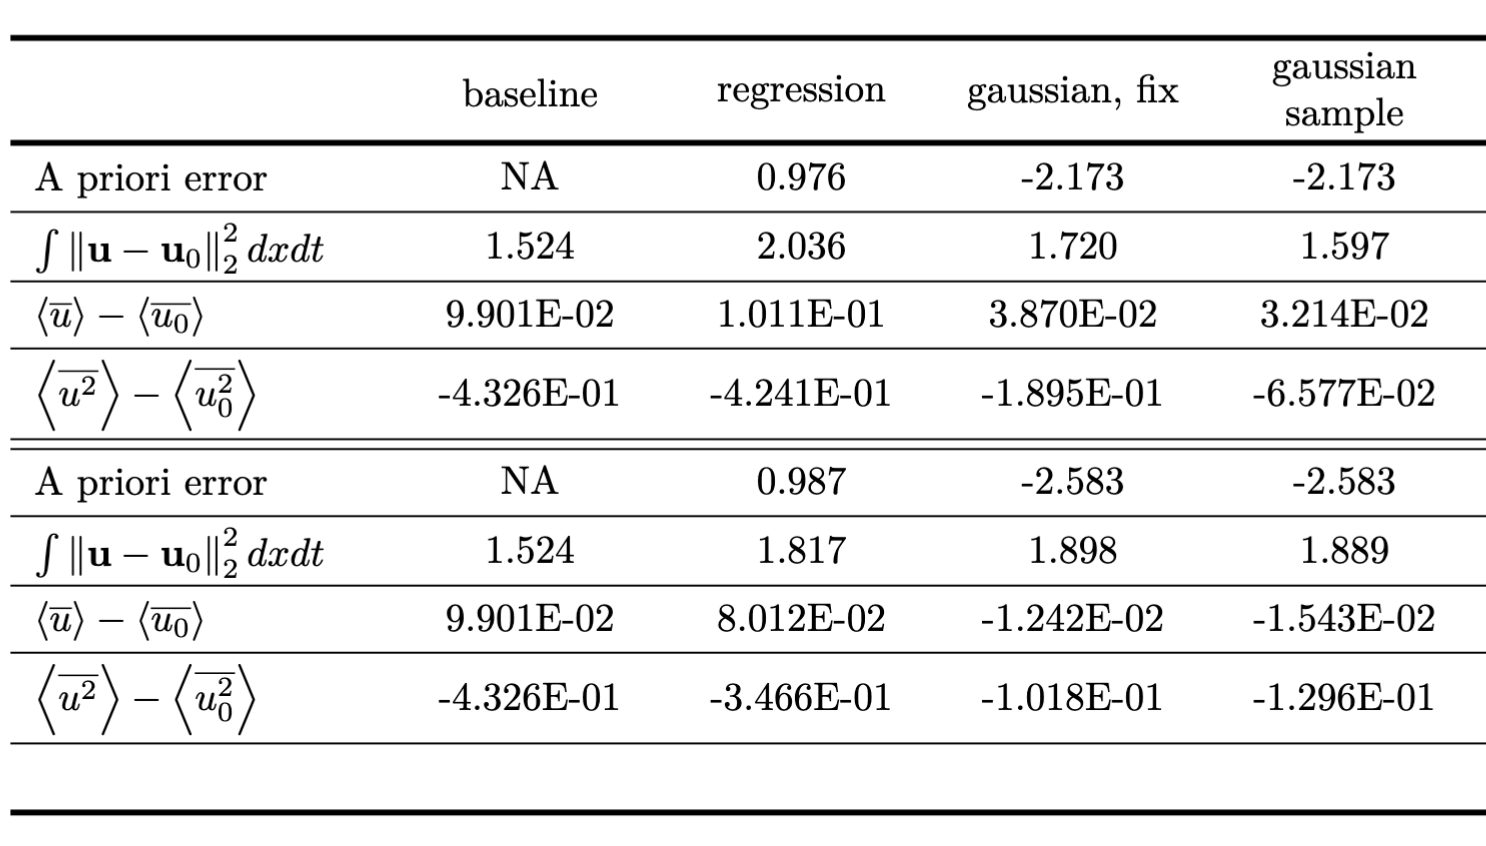
\includegraphics[width=.7\textwidth]{fig/table.jpg} 
	\end{figure}
\end{frame}

\begin{frame}{First stage NS equation results}
	\begin{equation*}
		\text{corr}(t) = \frac{\langle u^{\text{c}}(\cdot, t), \overline{u^{\text{f}}}(\cdot, t) \rangle}{\norml u^{\text{c}}(\cdot, t) \normr_2 
		\norml \overline{u^{\text{f}}}(\cdot, t) \normr_2},
	\end{equation*}

	Our method can achieve a better temporal correlation with the fine-grid simulations
	comparing to the regression-based methods.
	\begin{figure}[ht] 
		\centering 
		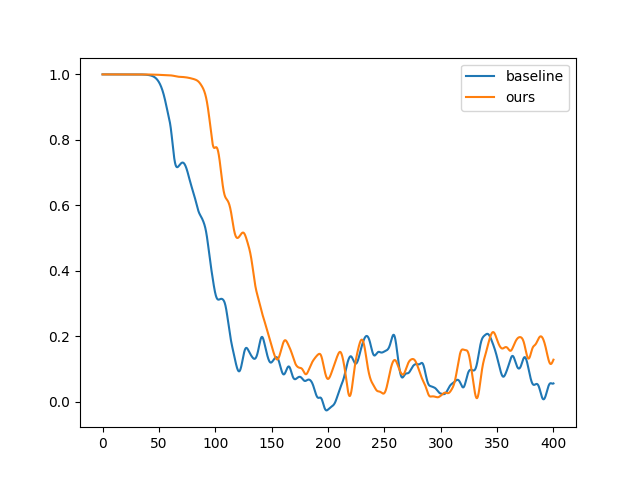
\includegraphics[width=.5\textwidth]{fig/sim_ks_correction_ols_unet_corr.png} 
	\end{figure}
\end{frame}


\begin{frame}{Conclusion}
	\begin{itemize}
		\item 1. We visualize and analyze the SGS modeling using 1D toy
		model of KS equation.
		\item 2. We propose a probabilistic ansatz for SGS modeling and
		corresponding training pipeline.
		\item 3. We show that the probabilistic ansatz can achieve a better
		temporal correlation with the fine-grid simulations comparing to the
		regression-based methods.
	\end{itemize}
\end{frame}


\begin{frame}{Future work}
	\begin{itemize}
		\item 1. Implement more expressive generative models for SGS modeling and
		investigate their performance.
		\item 2. Deploy to practical problems: Subgrid-scale modeling in large
		eddy simulation of the
		urban environment.
		\item 3. Theoretical understanding of the difference between
		regression-based and generative-based SGS modeling, especially in different
		application scenarios such as CFD and MD.
	\end{itemize}
\end{frame}


\begin{frame}{References and advertisement}
	{\tiny
	\begin{itemize}
		\item 1. Zhao, Jiaxi, and Qianxiao Li. "Mitigating Distribution
		Shift in Machine Learning–Augmented Hybrid Simulation." SIAM Journal
		on Scientific Computing 47.2 (2025): C475-C500.
		\item 2. Zhao, Jiaxi, Sohei Arisaka, and Qianxiao Li. 
		"Generative subgrid-scale modeling." ICLR 2025 Workshop on Machine Learning Multiscale Processes. 2025.
		\item 3. Code repository: \url{https://github.com/jiaxi98/ml4dynamics}.
	\end{itemize}
	}

	\textbf{I am looking for both industrial and academic positions starting from this year, collaborations and
	discussions are also warmly welcome!}
	\begin{itemize}
		\item Email: \href{mailto:jiaxi.zhao@u.nus.edu}{jiaxi.zhao@nus.edu.sg}; 
		WeChat:
		\begin{figure}[ht] 
			\centering 
			
\includegraphics[width=.3\textwidth]{fig/qrcode.jpg} 
		\end{figure}
	\end{itemize}
\end{frame}


% \begin{frame} % Use [allowframebreaks] to allow automatic splitting across slides if the content is too long
%     \frametitle{References}
 
%     \begin{thebibliography}{99} % Beamer does not support BibTeX so references must be inserted manually as below, you may need to use multiple columns and/or reduce the font size further if you have many references
%         \footnotesize % Reduce the font size in the bibliography
 
% 		\bibitem[BDI]{bdi}
% 		M. Benjamin, S. Domino, and G. Iaccarino
% 		\newblock Neural Networks for Large Eddy Simulations of Wall-bounded Turbulence: Numerical Experiments and Challenges
% 		\newblock \emph{The European Physical Journal E}

% 		\bibitem[Zhao 2024]{ds}
%         J. Zhao and Q. Li (2024)
%         \newblock Mitigating Distribution Shift in Machine Learning-augmented Hybrid Simulation
%         \newblock \emph{Arxiv preprint https://arxiv.org/pdf/2401.09259}

%         \bibitem[S.A. and Q.L., 2024]{nigbms}
%         S. Arisaka and Q. Li (2024)
%         \newblock Accelerating Legacy Numerical Solvers by Non-intrusive Gradient-based Meta-solving
%         \newblock \emph{International Conference on Machine Learning 2024}
 
        
%     \end{thebibliography}
% \end{frame}


% backup slide
\begin{frame}{KS Statistics}
	\begin{figure}[ht] 
		\centering 
		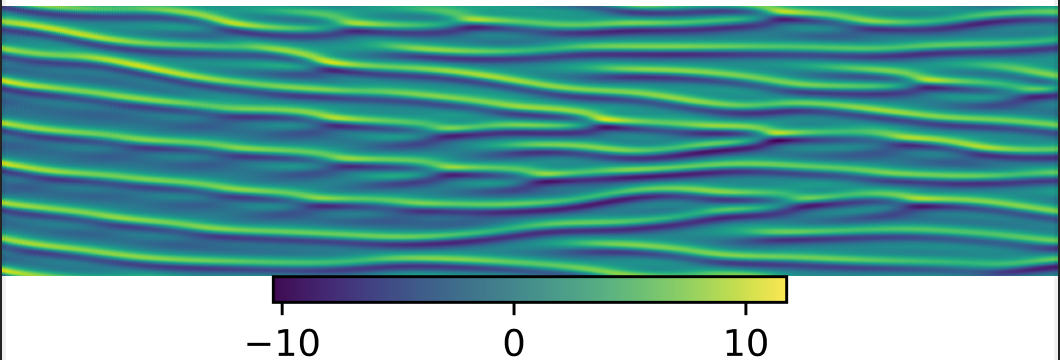
\includegraphics[width=.6\textwidth]{fig/ks.jpg} 
		\label{fig:stats}
	\end{figure}
	\begin{figure}[ht] 
		\centering 
		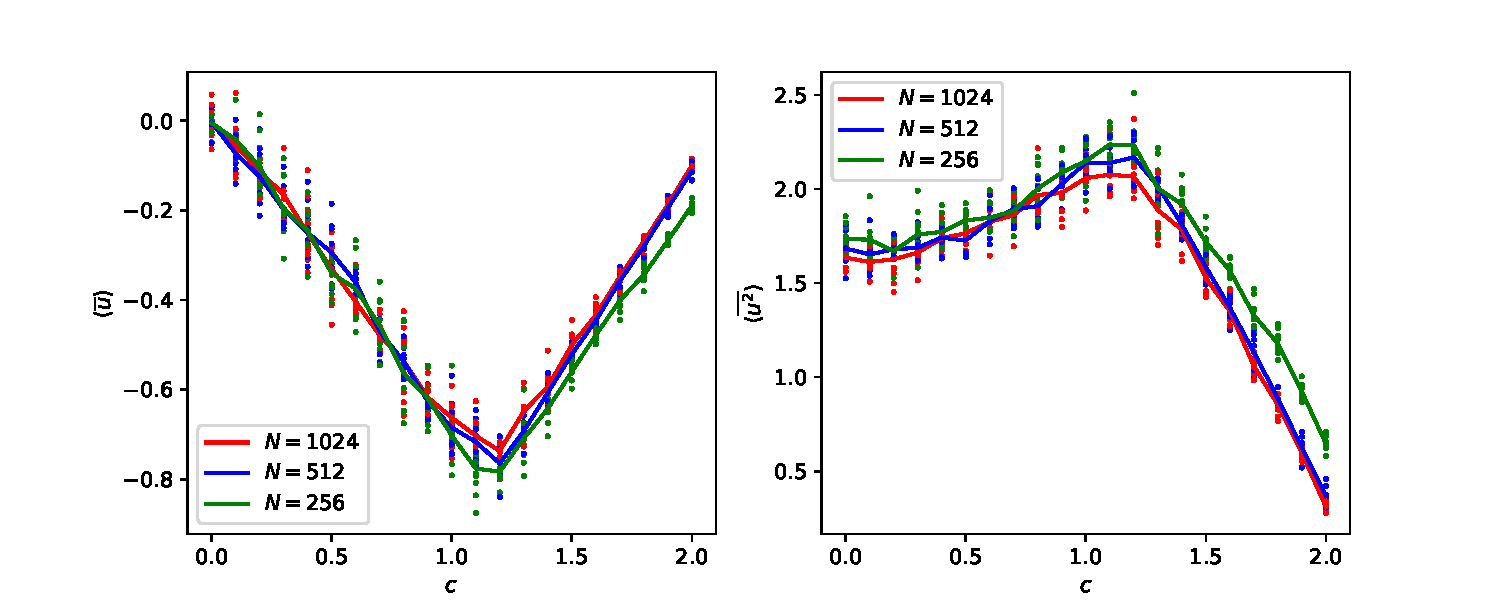
\includegraphics[width=.8\textwidth]{fig/ks_c_stats.pdf} 
		\label{fig:stats}
	\end{figure}
\end{frame}

\end{document}